% \section{Case Study: Environmental Justice in Rulemaking} 
I explore the role of public comments in rulemaking by focusing on their role in the environmental justice movement. Environmental justice concerns focus on the unequal access to healthy environments and protection from harms caused by things like pollution and climate change. The ways in which agencies consider environmental justice highlights how rulemaking has distributive consequences, how the public comment process creates temporary political communities, and how claims raised by activists are addressed. %, conditional upon their alignment with agency missions. 

Examining over 20,000 rulemaking processes at agencies known to address environmental justice concerns, I find that when public comments raise environmental justice concerns, these concerns are more likely to be addressed in the final rule. In this preliminary analysis, however, the number of comments mobilized is not related to success. While we cannot infer that agencies addressing environmental justice concerns is caused by the public comments themselves, comments may be a good proxy for lobbying in general. Furthermore, the correlation between raising environmental justice and policy changes is largest and most significant in agencies with missions focused on environmental and distributional policy, i.e. the kinds of bureaucrats who we may expect to have institutional and cognitive processes primed to be most responsive to environmental justice concerns.

This case illustrates the way that activists use public comments to inject ideas directly into the rulemaking process. I focus on the environmental justice movement because it offers a broad but tractable scope for analysis and shows what is at stake in the politics of rulemaking.  How rules consider environmental justice issues illustrates how rulemaking constructs a political community of ``relevant'' stakeholders and ``appropriate'' criteria to evaluate policy consequences. Thus, the idea of environmental justice is an example of how social movements can mobilize norms and evaluative frameworks that are connected to organizational identities, mission, and reputations and that have implications for bureaucratic decisions. 

The use of an environmental justice frame does not always imply the same communities of concern. Environmental justice emerged out of movements against environmental racism, especially the disposal of toxic substances in communities of color \citep{Bullard1993}. However, the term quickly took on a wider array of meanings, encompassing any marginalized group. In 1994 the Bill Clinton signed an Executive order on Environmental Justice that required all parts of the federal government to make ``addressing disproportionately high and adverse human health or environmental effects of programs, policies, and activities on minority populations and low-income populations'' a core aspect of their mission. This meant considering disproportionate effects during rulemaking.

Fundamental definitions of the public good and minority rights are implicit in agency rules. The public comment process offers an opportunity to protest these definitions. Protest is one way that marginalized groups can communicate opinions on issues to government officials \citep{Gillion2013}. %Gillion2015,
In the case of the EPA's Mercury Rules, two such issues were decisive. First, as with many forms of pollution, mercury-emitting power plants are concentrated in low-income, often non-White communities. Second, certain populations consume much more locally-caught freshwater fish, a major vector of Mercury toxicity. Studies inspired by the political controversy around the Mercury Rules found high risk among communities included ``Hispanic, Vietnamese, and Laotian populations in California and Great Lakes tribal populations (Chippewa and Ojibwe) active on ceded territories around the Great Lakes'' (EPA 2012). Thus the standards that EPA chooses are fundamentally dependent on whom the regulation aims to protect: the average citizen, local residents, or fishing communities. This decision has disparate effects based on race and class because of disparate effects based on geography and different cultural practices. Such disparate impacts are often called environmental justice issues.

In December 2000, when the EPA first announced its intention to regulate Mercury from power plants, the notice published in the Federal Register did not address environmental justice issues such as the disparate effects of mercury on certain populations. Risks were only discussed in reference to ``the U.S. population'' (EPA 2000). When the first draft rule was published, it only discussed the effects of the rule on regulated entities, noting that ``Other types of entities not listed could also be affected'' (EPA 2002). Commenting on this draft, Heather McCausland of the Alaska Community Action on Toxics (ACAT) wrote:
\begin{quotation}
``The amount of methyl-mercury and other bioaccumulative chemicals consumed by Alaskans (especially Alaskan Natives) could potentially be much higher than is assumed...The Alaska Native mortality rate for babies which according to the CDC is 70\% higher than the United States average. Indigenous Arctic \& Alaskan Native populations are some of the most polluted populations in the world (http://www.amap.no/). Global transport \& old military sites contaminate us too''
\end{quotation}

After receiving hundreds of thousands of comments and pressure from tribal organizations, a revised proposed rule echoed McCausland's comment noting that ``Some subpopulations in the U.S., such as Native Americans, Southeast Asian Americans, and lower-income subsistence fishers, may rely on fish as a primary source of nutrition and/or for cultural practices. Therefore, they consume larger amounts of fish than the general population and may be at a greater risk of the adverse health effects from Hg due to increased exposure'' (EPA 2004). 

After nearly a million additional public comments, a revised proposed rule ultimately included five pages of analysis of the disparate impacts on "vulnerable populations" including ``African Americans,'' ``Hispanic,'' ``Native American,'' and ``Other and Multi-racial'' groups (EPA 2011). In the final rule, the language of ``vulnerable populations '' was replaced with ``minority, low income, and indigenous populations'' (EPA 2012). EPA had also conducted an analysis of sub-populations with particularly high potential risks exposure due to high rates of fish consumption as well as an additional analysis of the distribution of mortality risk by to race.

Of this second round of comments, over 200 explicitly raised the environmental justice issues. The Little River Band of Ottawa Indians expressed the Tribe's ``frustration at trying to impress upon the EPA the multiple and profound impacts of mercury contamination from a Tribal perspective. Not to mention the obligations under treaties to participate with tribes on a “Government to Government” basis. At present, no such meetings have occurred in any meaningful manner with EPA Region V, the EPA National American Indian Environmental Office, nor the State of Michigan’s Department of Environmental Quality.'' They conclude that "Although EPA purported to consider environmental justice as it developed its “Clean Air Mercury Rule,” it failed utterly. In this rulemaking, EPA perpetuated, rather than ameliorated, a long history of cultural discrimination against tribes and their members'' (Sprague 2011). Did comments like these play a role in EPA's changed analysis of who Mercury limits should aim to protect?

Given the many potential sources of influence, it may be difficult to attribute causal effects of particular comments on a given policy. However, comments may serve as a good proxy for the general mobilization of groups and individuals around an administrative process, and it is not clear why EPA would not address environmental justice in the first draft of a rule and then add it to subsequent drafts in the absence of activists mobilization. Electoral politics does not offer an easy explanation. The notice proposing the Mercury Rule was issued by the Clinton administration, the same administration that issued the Executive Order on Environmental Justice, and the subsequent drafts that did address environmental justice issues were published by the Bush administration, which had a more contentious relationship with environmental justice advocates, while Republicans controlled both houses of Congress. The expansion of the analysis from one draft to the next seems to be in response to activist pressure. 

Mobilization around ideas like environmental justice may even affect policy discourse when agency administrators are explicitly hostile to the cause. For example, in an October 2017 proposed rule to repeal restrictions on power plant pollution, the Trump EPA acknowledges that ``low-income and minority communities located in proximity to [power plants] may have experienced an improvement in air quality as a result of the emissions reductions.'' Because the Executive Order requires attention to environmental justice and because the Obama EPA discussed it when promulgating the rule, the environmental justice cannot safely be ignored. However,  the Trump EPA contends, the Obama EPA ``did not address lower household energy bills for low-income households [and that] workers losing jobs in regions or occupations with weak labor markets would have been most vulnerable'' (EPA 2017). As of \today, this proposed rule has received over 150,000 public comments. 

Tracing ideas like environmental justice through the rulemaking record may offer one way to study the mechanisms by which social movements do or do not influence bureaucratic policymaking. Specifically, if rules are proposed without attention to environmental justice concerns, but environmental justice concerns are raised in the public comments and then appear in the final policy, this may be evidence that mobilization mattered.

Environmental justice is certainly not the only way to observe such effects, but it has some convenient properties. First, policies framed as ``environmental'' issues are, unlike issues like issues like civil rights and immigration, inconsistently racialized and, unlike issues like taxes and spending, inconsistently focus on \textit{distributions} of costs and benefits. Despite almost always having disparate impacts, an environmental frame often creates a human-environment distinction and shifts attention to non-human objects such as air, water, food, or landscapes and away from the distribution of access to these objects or protection from them when they are contaminated. Second, compared to other ideas around which people mobilize, ``environmental justice'' is a fairly distinctive phrase. Most people who use this phrase share a general definitional foundation. Third, this phrase is fairly common when the idea is being discussed, i.e. there are not many synonyms and groups raising equity concerns on ``environmental'' issues commonly refer to environmental justice.  Many who use the narrower, related term ``environmental racism'' also use ``environmental justice'' in their advocacy.  Finally, the term is relevant to rulemaking records in particular because of an Executive Order issued in 1994 by President Clinton "Federal Actions to Address Environmental Justice in Minority Populations and Low-Income Populations" which required all agency actions and policies to consider environmental justice implications. This does not mean that all draft or final rules do so, but when they do, they tend to cite the executive order and explicitly discuss environmental justice. For the same reason, commenters, especially sophisticated ones, who critique draft rules also use the cite this executive order and use this language. 

\subsection{Data}
In order to examine whether the environmental justice movement's mass mobilization of letter-writing influences the discourse around policies, I use the text of draft rules, public comments, and final rules retrieved from regulations.gov.  Figure \ref{fig:ej} compares the use of the term ``environmental justice'' in draft policies, public comments on these drafts, and the final versions of the policies. I collected all documents from the website regulations.gov and selected 58,789 that use the phrase ``environmental justice.'' This includes %4,141 notices of intent to propose a rule, 
5,109 proposed rules, 17,539 public comments on these %notices and 
proposed rules, and 10,418 final rules. I then added all draft and final rules from all 35 agencies that have published at least one rule addressing environmental justice, an additional 40,096 documents.\footnote{This may be an over-inclusive sample and in future work, I may attempt to refine this sample to rules that plausibly relate to environmental justice issues.}  % CORRECT THESE NUMBERS 

Notably, more than twice as many final rules as proposed rules contain the phrase ``environmental justice.'' This suggests a systematic element in how agency policymakers are revising draft rules and responding to public comment. Below, I investigate the extent that this change from the draft to final policy is related to environmental justice issues being raised in the public comments. 

\begin{figure}[h!]
\caption{Number of Rules where Environmental Justice Appears in the Record (Left) and Number of Comments per Notice or Proposed Rule (Right). Text indicates the agency for the most commented on rules.}
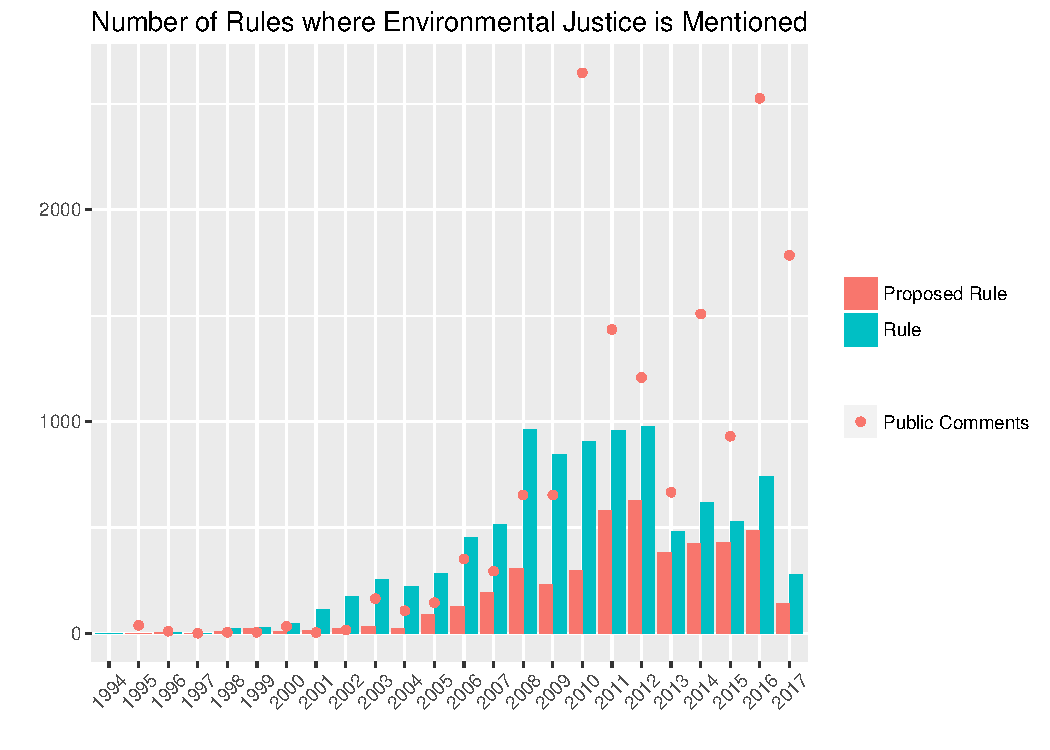
\includegraphics[width = 3.5in]{eandj_hist.pdf}
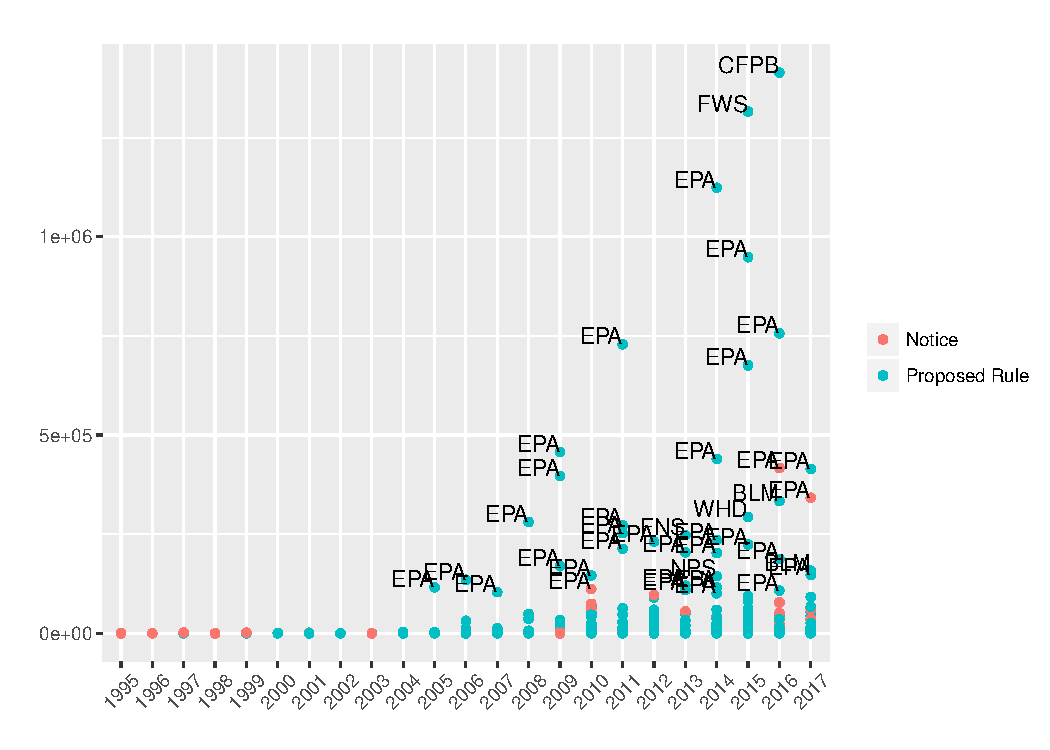
\includegraphics[width =3.5in]{eandj_comments.pdf}
\label{fig:ej}
\end{figure}

Figure \ref{fig:ej} shows that the number of rules and comments increasing over time. This may reflect increased salience of this concept, but it may primarily be the result of the increasing prevalence of searchable texts.  Similarly, the increased number of rules where comments mention environmental justice may reflect growth in the movement but also may reflect more overall comments as technology has made commenting easier. Testing the hypotheses that comments raising environmental justice concerns are related to specific rules where environmental justice is addressed in the final but not in the draft requires rule-specific analysis. 

What we can say from Figure  \ref{fig:ej}  is that each year, more final rules directly address environmental justice when their draft did not. Additionally, there are many rules where environmental justice is mentioned in the public comments and not in the draft. Recently, there are also many rules where environmental justice is raised in the comments but does not make it into the final draft.\footnote{Note that, because not all comments are searchable, this is an underestimate of the number of comments mentioning environmental justice, so we cannot conclude that before 2010, rules were mentioning environmental justice when the comments had not. Additionally, this does not include comments like those of the Bishops who raise justice issues but do not use the phrase ``environmental justice.''} 

% \subsection{Next Steps}
%With these data in hand, the next step is to match each draft and final rule to identify how each changed and to match each comment to its rule to see if the observed changes were suggested in comments. 

\subsection{Second-order Representation} Before analysis of whether comments matter, I briefly describe who these commenters are. This is what \citet{Seifter2016UCLA} calls ``second-order'' representation. It is insufficient to know which groups participate. We also need to know who these groups represent.

I  investigate who is raising environmental justice concerns in two ways. First, I  identify the top organizational commenters such as tribes, businesses, and nonprofits that are using environmental justice language and investigate who these groups represent. Second, for comments where a citizen signed their name, I  compare surnames to their racial and ethnic identity propensities with respect to the U.S. census. Together these two pieces of information allow me to comment on ``second order'' representation, i.e. not just the extent to which public comments relate to government policy, but the extent to which public comments are representative of the public and of the groups they claim to represent. 



\begin{table}[!h] 
  \caption{Organizations mobilizing mass comment campaigns mentioning "environmental justice"}
\centering
\begin{tabular}{rlll}
  \hline
 & Organization & Comments & Rules \\ 
  \hline
1 & Earthjustice & 1114782 & 28 \\ 
  2 & Natural Resources Defense Council &  340554 &  8 \\ 
  3 & Sierra Club &  349841 &  5 \\ 
  4 & Alliance for Climate Protection &  253867 &  5 \\ 
  5 & WE ACT for Environmental Justice &    2402 &  3 \\ 
  6 & CREDO &  112879 &  2 \\ 
  7 & Union of Concerned Scientists &   43559 &  2 \\ 
  8 & Earthworks &     308 &  2 \\ 
  9 & Communities for a Better Environment &      21 &  2 \\ 
  10 & Southern Company &       8 &  2 \\ 
  11 & Move On &  165948 &  1 \\ 
  12 & Care2 &   70450 &  1 \\ 
  13 & The Pew Charitable Trusts &   63769 &  1 \\ 
  14 & Hudson-Environmental Action &   35000 &  1 \\ 
  15 & Democracy for America &    4426 &  1 \\ 
  \end{tabular}
  \label{tab:orgs}
\end{table}

Table \ref{tab:orgs} shows the top 15 organizational commenters who used the phrase ``environmental justice'' in their comments, including all organizations who did so on more than one rule or mobilized more than 100,000 such comments. The six organizations responsible for mobilizing more than 100,000 comments and several others on the list are national nonprofit advocacy groups.  We Act and Communities for a Better Environment are both more community-based groups focusing primarily on environmental justice issues. Southern Company is the only corporation on the list
 
 The top mobilizer, Earthjustice, is primarily engaged in litigation on behalf environmental causes. Their website boasts 2.2 million supporters,  but it is not clear who they are or if they play any role in the advocacy strategy. A search on the website returns 360 results for "Environmental Justice," with the top results from staff biographies who work on more local or targeted work such as environmental conditions for the incarcerated, but the environmental justice language used on the main page is relatively mild. For example, ``We are fighting for a future where children can breathe clean air, no matter where they live'' \citep{Earthjustice2017}. The website does contain Spanish language content. 
 
 The Natural Resources Defense Council is similar to Earthjustice--a national nonprofit funded by donations and focused on litigation--but they also lobby. CREDO Action and MoveOn are more generic progressive mobilizers who lack a systematic focus on environmental justice issues, but occasionally leverage their very large membership lists to support campaigns environmental justice campaigns led by others \citep{MoveOn.org2017, CREDO2017}. The Alliance for Climate Protection is a more of an elite political group founded by former Vice President Al Gore. 
 
 We Act and Communities for a Better Environment both have environmental justice in their central mission statement. We Act was founded by community leaders in Harlem, NY, to fight environmental racisms and advocate for better air quality \citep{WEACT2017}. Communities for a Better Environment has projects throughout California but is particularly active in Oakland \citep{CBECAL2017CommunitiesEnvironment}. Much of the content of their website is in both English and Spanish. Both organizations focus primarily on ``low-income communities of color'' and thus frame their work with respect to race and class. While both organizations participated in national policymaking We Act is more focused on communities in Harlem and New York whereas Communities for a Better Environment casts a wider frame: "CBE’s vision of environmental justice is global--that’s why the organization continues to participate in such international efforts as the Indigenous Environmental Network and the Global Week of Action for Climate Justice" \citep{CBECAL2017}.
 
 The Southern Company comments are too few to count as mass mobilization. Companies do sometimes fund mobilization campaigns, but all of 8 of these comments were submitted by the Southern Company. Interestingly, the company repeatedly raises research into environmental justice concerns in order to frame these issues as a legitimate but unresolved scientific debate that is not yet conclusive enough to base regulations on: "People with lower SES are exposed to almost an order of magnitude more traffic near their homes (Reynolds et al., 2001), and live closer to large industrial sites and are exposed to more industrial air pollution (Jerrett et al., 2001). Legitimate health concerns must be addressed. But adopting standards with a scientific basis so uncertain that health improvement cannot be assured is not sound public health policy." Like many companies they claim to represent their customers as "electric generating companies and their customers are expected to bear much of the burden" of regulations \citep{Hobson2004}.
 
 With respect to second-order representation, it appears that the groups most often using the language of environmental justice may do so sincerely but do not themselves represent affected communities. Several groups representing local communities and led by community leaders have participated, but not nearly as often or with the same intensity as the ``big greens.'' This highlights the importance of resources as a condition for mobilizing. Not all groups who may benefit from political information are able to leverage it because they lack the resources to invest in a campaign. However, it may be the case that smaller, more member-driven groups join coalitions with groups with more resources who mobilize on their behalf. More work is needed to identify coalitions to assess this possibility.

 Finally, a third class of commenter raises environmental justice issues as a way to re-frame them as ongoing debates and thus undermine their urgency. I call this reason for engaging as ``breaking a perceived consensus.'' In a way, the fact that an energy company felt compelled to acknowledge and question environmental justice concerns suggests their importance for policy outcomes.

Next, I attempt to estimate the racial distribution of those who comment using environmental justice language. This can only be done for individuals who commented separately from mobilizing organizations and signed their full name on their comment. 
Figure \ref{ejcommentsbyrace} shows two ways of estimating the racial distribution of commenters who raise ``environmental justice'' concerns in their comments. Both methods use the reported racial identities associated with surnames as recorded in the 2010 census\footnote{I recode ``Hispanic'' as ``Latinx'' in both cases because the prediction method assumes a forced choice that includes ``Hispanic'' as a primary racial category} and are based on a limited sample of 327 commenters who signed their name with a surname matching census records.  The first is based on the proportion of people with a given surname that identified as belonging to each racial category (from this limited set of options). The estimated proportion of each race for this sample is simply the average of proportions identified with each surname. This is likely the most accurate way to represent the racial distribution of a set of surnames, but it does not assign specific individuals to racial categories. The second method does. It predicts the race of each individual in the sample based on their surname given the distribution of racial categories reported by people with that surname and the proportion of each race in the U.S. population. Thus, while a surname may be more common among people who identify as black rather than as white, there may still be more White people with that surname and this method would predict that the person is White. For this reason, the portion of individuals predicted to be White (right) is higher than in the probabilistic distribution (left). 

\begin{figure}[h!]
\caption{Probabilistic (Left) and Predicted (Right) Race from Census Surnames}
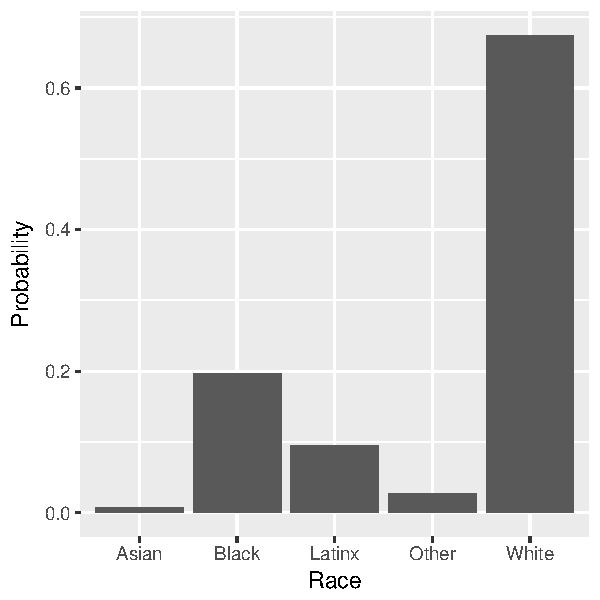
\includegraphics[width = 3in]{race_prob.pdf}
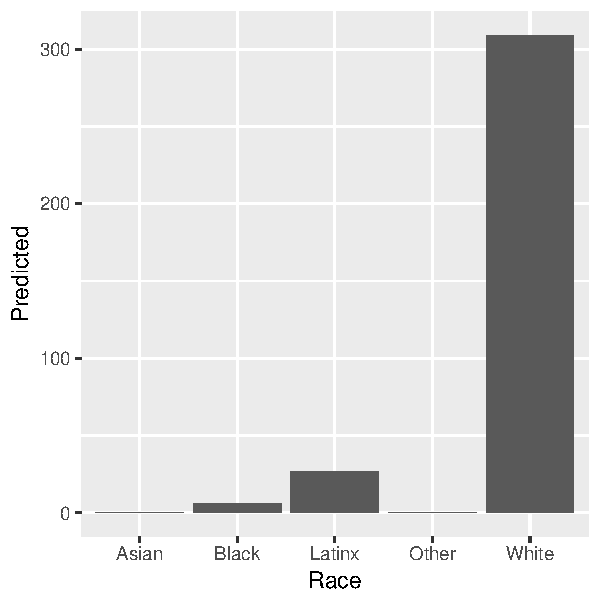
\includegraphics[width = 3in]{race_pred.pdf}
\label{ejcommentsbyrace}

\end{figure}

Compared to estimates from the 2010 census, this sample of commenters appears to be disproportionately Black and less than proportionately Latinx or Asian, with just slightly fewer Whites relative to the national population. This makes sense given that environmental justice theorizing and activism have been led by African American's \citep{Bullard1993}.

Figure \ref{ejwordsbyrace} shows the most common words used in comments with respect to the predicted race of each commenter in the sample. As there are very few predicted non-White commenters in the sample, it is unwise to infer too much from this figure. 


\begin{figure}[h!]
\caption{Common words used in comments mentioning ``environmental justice'' by predicted race}
\begin{tabular}{ccc}
White & Latinx & Black\\
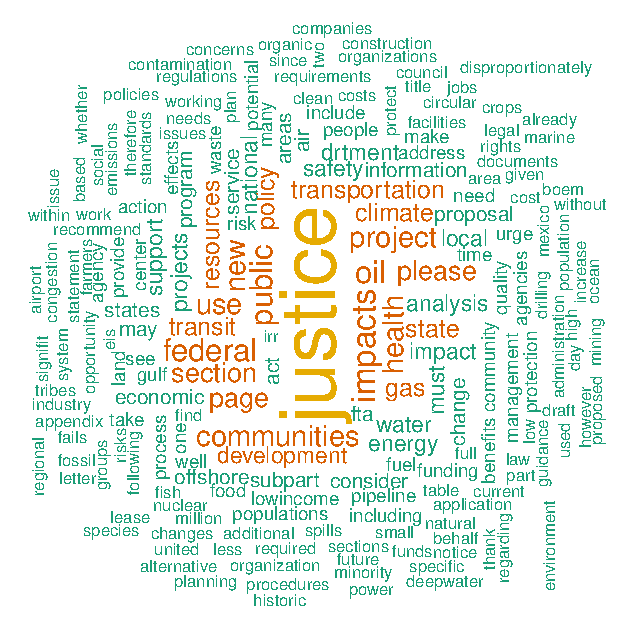
\includegraphics[width = 2in]{ej_white_words.pdf}
&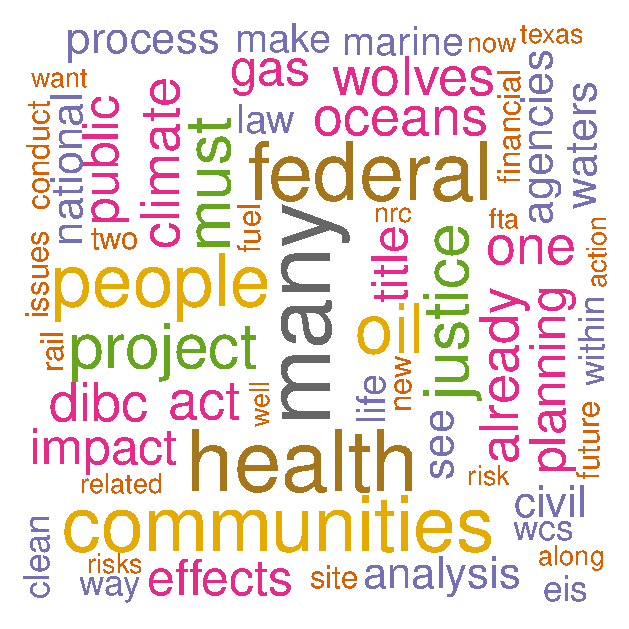
\includegraphics[width = 2in]{ej_latinx_words.pdf}
&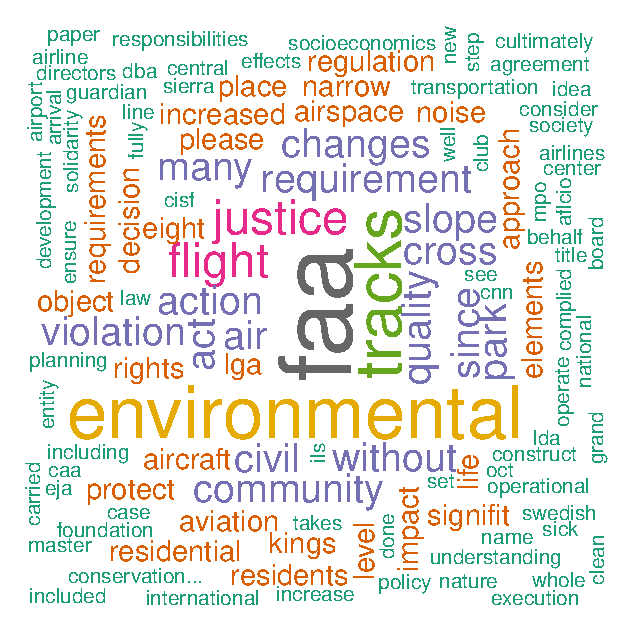
\includegraphics[width = 2in]{ej_black_words.pdf}
\end{tabular}
\label{ejwordsbyrace}
\end{figure}

% Time allowing I will also investigate different pathways to influence such as how rule-specific environmental justice concerns were raised in congressional hearings and reports. 


\subsection{Results: Are final rules more likely to address environmental justice after comments do so?}
This subsection presents preliminary results from an analysis of draft rules, comments, and final rules. Descriptively, figure \ref{ejwinrate} shows that in general, most rules that do not address environmental justice in the draft but these issues are raised in the comments, do not end up addressing them in the final version. It appears that it may have been the case in 2006 and 2007 but since then the number of rules receiving comments raising environmental justice concerns has grown while the number of rules that end up adding it has remained the same. Since 2015, there has been a decline in both the number of rules adding environmental justice and the number of rules where commenters demanded it, especially in 2017. One way to interpret figure \ref{ejwinrate} would be to say that commenters saw a potential ally in President Obama and increased their demands for environmental justice, but that these increased demands had little effect. However, a better approach would be to estimate a statistical model of the effect of comments on the change from draft to final rules. This is what I do.


\begin{figure}[h!]
\caption{Rules With Comments Addressing EJ on a Draft That Did Not}
\centering
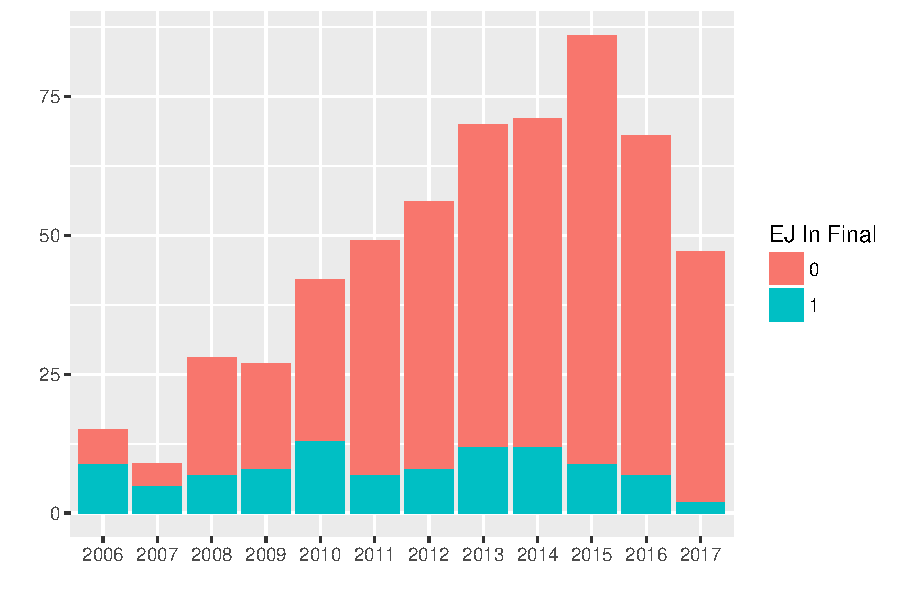
\includegraphics[width = 3.5in]{ej_win_rate.pdf}
\label{ejwinrate}
\end{figure}


For this preliminary analysis, I estimate a logit regression where the outcome is whether environmental justice was addressed in the final rule and the predictors are whether it was addressed in the draft rule, whether it was addressed in the comments, and the total number of comments received. 

\begin{align*}
  \hat{EJ in Final} = \Bigg\{ \begin{array}{lll}
    1 & if &  \beta_0 + \beta_1 EJ in Draft + \beta_2 EJ in Comments + \beta_3 Total Comments  + \epsilon > 0\\
0 & otherwise &  
  \end{array}
\end{align*}

As logit coefficients are not easily interpretable, I calculate predicted probabilities for the types of rules of interest, i.e. rules where environmental justice was not raised in the draft, \textit{EJinDraft}=0. Figure \ref{ejpredicted} shows the predicted probability of a final rule addressing environmental justice when the draft rule did not for all agencies that have ever published a rule addressing environmental justice (left) and the EPA alone (right). The EPA accounts for nearly two-thirds of the cases where environmental justice is raised in the comments on a draft rule that did not address it. The total number of comments mentioning ``environmental justice'' had a substantively small and statistically insignificant effect on policy. As the flat lines on both figures show, the predicted probability of adding the phrase ``environmental justice'' does not increase with the number of comments. Environmental justice being raised in any one comment does have a statistically significant and substantively large effect. 

Overall the probability across all agencies of adding environmental justice increases from under 2\% to about 9\%. At the EPA, the probability triples from about 6\% to about 18\%. 


\begin{figure}[h!]
\caption{Proposed Rules Not Addressing Environmental Justice (Left: All agencies. Right: Environmental Protection Agency)}
\centering
\noindent
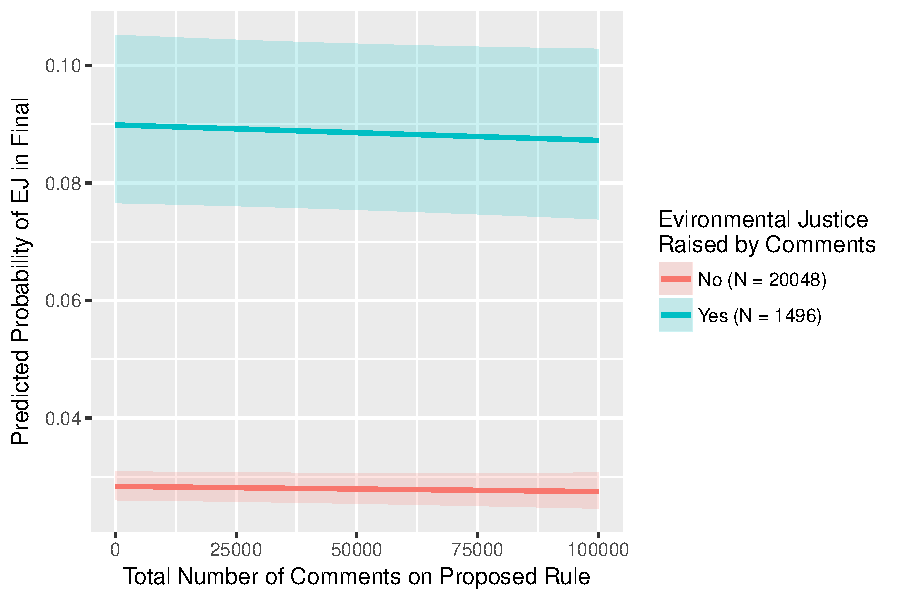
\includegraphics[width = 3.2 in]{ej_prob_env_nprms.pdf}
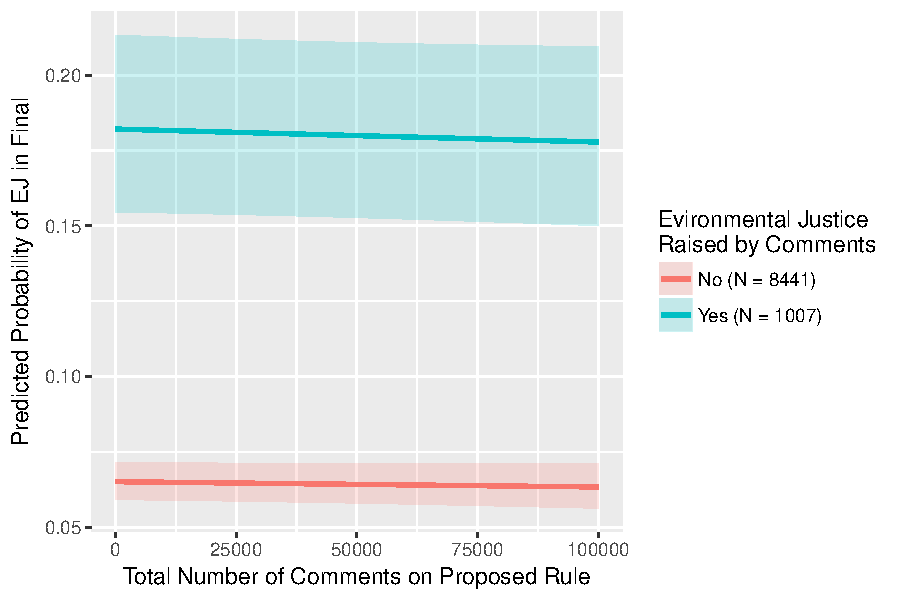
\includegraphics[width = 3.2 in]{ej_prob_epa_nprms.pdf}
\label{ejpredicted}
\end{figure}

To examine the degree to which this generalizes across agencies, figure \ref{ejlogitagencies} presents predicted probabilities modeled for each agency, showing that the range of predicted probabilities is systematically higher when environmental justice, but with varying degrees of confidence. There is considerable variation among agencies. Point estimates are only shown for agencies where confidence intervals do not overlap. Only a few agencies have statistically significant different estimates, but the agencies where effects are largest are exactly the agencies we would expect to be influenced by comments raising environmental justice concerns, i.e. agencies that deal with environmental issues with distributive consequences. 


\begin{figure}[h!]
\caption{Proposed Rules Not Addressing Environmental Justice}
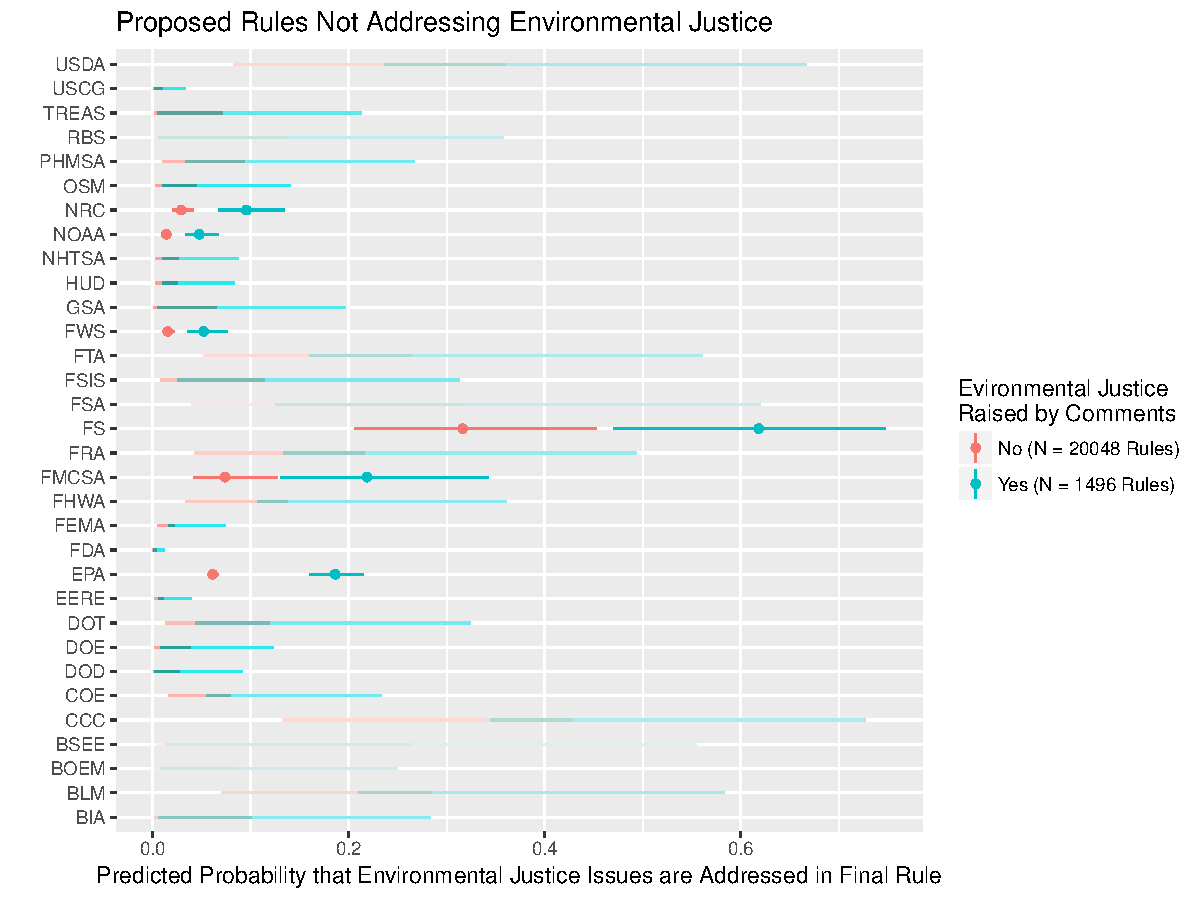
\includegraphics[width = \textwidth]{ej_prprob_by_agency.pdf}
\label{ejlogitagencies}

\end{figure}

As the EPA accounts for the largest portion of the data, we are most confident in this result, but the EPA is not the agency with the largest predicted effects. The Forest Service has a predicted 30\% difference between rules that do and do not receive comments raising environmental justices concerns. This may be because the forest service is mainly in the business of managing forests, leasing timber rights, and controlling wildfires. These types of decisions may have acute distributional effects that may not be the initial focus of the agency. Once raised, however, addressing such effects fits squarely in their mission. Though not statically significant the Department of Agriculture and Bureau of Land Management, who make similar kinds of decisions, are also susceptible to environmental justice claims. Similarly, the Federal Railroad Administration, Department of Transportation, Federal Highway Administration, Federal Motor Carrier Safety Administration, and the Federal Transportation Administration (which aids local transportation projects) all have large probability distributions. These agencies are making decisions about infrastructure projects with implications for neighborhood environments and air quality. Environmental justice may often come up, but there may be a lot of variation in whether the agency then decides if they are relevant to transportation policies and projects that are primarily about neither environmental nor justice concerns. 

Research agencies, including the National Research Council, National Oceanographic and Atmospheric Administration and Fish and Wildlife Service all had statistically significant but small spreads. In these cases, we can be confident of the correlation but understand that it is a rare occurrence, which makes sense if most research does not have direct environmental justice consequences, but agencies are open to adding analysis of these issues if when they are raised. 

\subsection{Conclusion}
This analysis has illustrated the importance of ideas in policymaking and cross-sectional statistical results suggest that when issue frames like environmental justice are raised there is a higher probability that policymakers consider the effects on marginalized populations. Importantly this relationship seems to be conditional on an institutional environment that is predisposed to such an analysis. Furthermore, it is important to note that the policy outcomes suggested by environmental justice analysis depend on how minority populations are defined. In some cases, those raising environmental justice concerns present it as an issue of wealth or income inequality, leading policy to account for disparate impacts on low-income populations. In other cases, groups raise claims rooted in cultural practices, such as fish consumption among certain tribes. As occurred in the Mercury Rule, the analysis in subsequent drafts of the policy used evaluative criteria specific to these communities. 

The ability of a frame like environmental justice to construct certain populations as deserving of consideration means that policy outcomes will depend on the specific environmental justice concerns raised. In this respect, second-order representation may become important. National  advocacy organizations may frequently request that regulators protect ``all people'' or even ``low-income communities of color.'' However, this more generic advocacy may not lead to the same outcomes as groups that present specific local environmental justice grievances that are unique to a community. In between generic progressive advocacy organizations and community-based organizations are organizations like Earthjustice who, despite their national focus, frequently engaged in community-specific litigation and thus raise these local concerns in national policymaking. 

In the end, the above analysis offers some clarity on a poorly understood but important mechanism of American policymaking. It offers some hope that citizen opinions may be heard through direct democracy institutions built into bureaucratic policymaking.  The examination of second-order participation validates some of the skepticism about who participates. It is elite groups who participate, even with respect to an issue like environmental justice. However, government responsiveness does not seem to depend on mass mobilization or elite support. Compared to cases where environmental justice issues were not raised, when they are, we see a significantly higher probability that they will be addressed by policymakers. 